% =====================================================================
%  research-paper-writing 스킬을 적용한 4쪽 한국어본 컴파일 래퍼.
%  템플릿 요구사항(00_템플릿_요구사항_정리.md): sigconf, CCSXML+ccsdesc, keywords,
%  모든 figure 에 \Description, booktabs, 세로줄 금지, ACM-Reference-Format.
%
%  컴파일 (paper-icaif26/ 에서):
%    xelatex build-ko-4p && bibtex build-ko-4p \
%      && xelatex build-ko-4p && xelatex build-ko-4p
% =====================================================================

% 제출본에서는 nonacm 을 제거하고, CFP 가 익명심사를 요구하면 anonymous 를 추가한다.
\documentclass[sigconf,nonacm]{acmart}

\IfFileExists{kotex.sty}{\usepackage{kotex}}{%
  \usepackage{fontspec}%
  \IfFontExistsTF{Noto Serif CJK KR}{%
    \setmainfont{Noto Serif CJK KR}[BoldFont={Noto Serif CJK KR Bold},
                                    ItalicFont={Noto Serif CJK KR},
                                    BoldItalicFont={Noto Serif CJK KR Bold}]%
    \setsansfont{Noto Sans CJK KR}[BoldFont={Noto Sans CJK KR Bold},
                                   ItalicFont={Noto Sans CJK KR},
                                   BoldItalicFont={Noto Sans CJK KR Bold}]%
    \setmonofont{Noto Sans Mono CJK KR}[Scale=0.92]%
  }{\setmainfont{Noto Serif CJK JP}\setsansfont{Noto Sans CJK JP}}%
  \XeTeXlinebreaklocale "ko"%
  \XeTeXlinebreakskip = 0pt plus 0.1em%
}

\usepackage{booktabs}
\usepackage{graphicx}
\usepackage{amsmath}
\usepackage{array}
\usepackage{placeins}
\setlength{\emergencystretch}{1em}

% tabular 내부에서 행 조각 파일을 읽기 위한 원시 \input
\makeatletter
\newcommand{\inputrows}[1]{\@@input #1 }
\makeatother

\settopmatter{printacmref=false,printfolios=true}
\setcopyright{none}

\AtBeginDocument{%
  \renewcommand{\figurename}{그림}%
  \renewcommand{\tablename}{표}%
}

\begin{document}

\title{집계 거래 흐름에서 투자자 유형별 행동계수의 표본 안정성}
\subtitle{4단계 검증을 통한 대칭 선호복원}

\author{저자명}
\affiliation{\institution{소속기관}\city{서울}\country{대한민국}}
\email{author@example.com}
\renewcommand{\shortauthors}{저자명}

\begin{CCSXML}
<ccs2012>
<concept>
<concept_id>10010405.10010455.10010461</concept_id>
<concept_desc>Applied computing~Economics</concept_desc>
<concept_significance>500</concept_significance>
</concept>
<concept>
<concept_id>10003752.10010070.10010071.10010261</concept_id>
<concept_desc>Theory of computation~Machine learning theory</concept_desc>
<concept_significance>300</concept_significance>
</concept>
</ccs2012>
\end{CCSXML}

\ccsdesc[500]{Applied computing~Economics}
\ccsdesc[300]{Theory of computation~Machine learning theory}

\keywords{투자자 유형별 수급, 벌점 회귀, 표본 안정성, 조합형 정화 교차검증, 행동재무}

\maketitle

% =====================================================================
%  research-paper-writing 스킬을 적용한 SPR 4쪽 한국어본.
%  영문 개선본과 수식, 수치, 인용, 주장 범위를 일치시켰다.
%  그림: fig4p_forest_no_v5.pdf, fig4p_prediction.pdf.
% =====================================================================

\section{방법: 대칭 선호복원}
\label{sec:method}

SPR은 공통 사양 아래에서 투자자 유형을 비교하도록 설계되었다. 먼저 다음 날의 순매수
행동을 정의하고, 세 가지 후보 행동 채널과 두 가지 시장 조건을 구성한 뒤, 모든 유형에
동일한 조건부 선형모형을 추정한다. 네 가지 검증 절차는 추정된 부호가 재표집 방식,
예측 시점의 순서, 추정량을 바꾸어도 유지되는지를 확인한다. 이 체계를
\emph{대칭 선호복원}(Symmetric Preference Recovery, SPR)이라 부른다. 복원된 계수는
집계 수급의 조건부 연관을 나타낼 뿐 구조적 선호를 뜻하지 않는다.

\subsection{행동 예측 문제}
\label{sec:setup}

투자자 유형 집합을
$\mathcal I=\{\text{외국인},\text{기관},\text{개인}\}$이라 하자. 유형 $i\in\mathcal I$의
$t$일 총매수금액과 총매도금액을 각각 $V^{buy}_{i,t}$와 $V^{sell}_{i,t}$라 두고,
정규화된 순매수 행동을
\begin{equation}
u_{i,t}=\frac{V^{buy}_{i,t}-V^{sell}_{i,t}}{V^{buy}_{i,t}+V^{sell}_{i,t}}\in[-1,1]
\label{eq:action}
\end{equation}
로 정의한다. 이 비율은 순매수를 총거래금액으로 조정하여 방향과 강도를 함께 보존한다.
예측 대상은 $a_{i,t+1}=u_{i,t+1}$이고, 입력 상태 $s_{i,t}=(x_{i,t},C_t)$에는 $t$일까지
관측된 정보만 포함한다.

세 유형은 동일한 특징벡터 $x_{i,t}\in\mathbb R^3$, 시장 컨텍스트
$C_t\in\mathbb R^2$, 모형 사양을 공유하며 파라미터만 별도로 추정한다. 따라서 유형별
예측변수를 따로 부여하지 않고도 적합 계수를 직접 비교할 수 있다.

\subsection{상태 특징과 시장 컨텍스트}
\label{sec:features}

상태벡터 $x_{i,t}=(x^{mom}_{t},x^{cross}_{i,t},x^{uw}_{i,t})^\top$는 최근 가격 움직임,
다른 유형의 시차 수급, 집계 손실구간이라는 세 후보 채널을 나타낸다.

\textbf{최근 가격 움직임.}
$P_t$를 삼성전자 종가라 하고, 사전에 정한 20일 로그수익률
\[
x^{mom}_{t}=\log(P_t/P_{t-20})
\]
을 사용한다. 계수가 양수(음수)이면 추세추종(역추세) 행동과 부호가 일치한다
~\cite{grinblatt2000investment,choe1999foreign}.

\textbf{다른 투자자 유형의 시차 수급.}
$i$를 제외한 두 유형을 $j,k$라 할 때,
$x^{cross}_{i,t}=(u_{j,t-1}+u_{k,t-1})/2$로 정의한다. 행동을 한 시점 지연하면 같은
거래일 투자자 수급 사이의 기계적 상쇄가 배제된다. 이 특징은 유형 간 시차 관계를
측정하며, 기관 내부 군집행동의 직접 검정은 아니다~\cite{lakonishok1992impact}.

\textbf{집계 손실구간.}
이 특징은 보유 중인 재고가 최근 거래가격보다 낮은지를 근사한다.
$Q^b_{i,t}$와 $Q^s_{i,t}$를 총매수ㆍ총매도 수량, $M^b_{i,t}$와 $M^s_{i,t}$를 대응하는
거래금액이라 하자. $Q^b_{i,t}>0$이면 매수 VWAP은
$P^b_{i,t}=M^b_{i,t}/Q^b_{i,t}$이다. 아래 재귀식에서는 공통 첨자 $(i,t)$를 생략하고
$[v]_+=\max(v,0)$로 쓴다.
\begin{equation}
\begin{aligned}
\widetilde H&=\rho H_{t-1}, & H&=[\widetilde H+Q^b-Q^s]_+,\\
O&=[\widetilde H-Q^s]_+, & N&=H-O,\\
\bar P&=\frac{O\bar P_{t-1}+NP^b}{H},&
P^{vwap}&=\frac{M^b+M^s}{Q^b+Q^s}.
\end{aligned}
\label{eq:cost}
\end{equation}
$\widetilde H$는 $t$일로 이월된 감가 재고, $O$는 매도 후 남은 기존 재고, $N$은 새로
유지된 재고, $H=O+N$은 총유효재고다. 이 재귀식은 유지수량과 평균단가 $\bar P$를 함께
갱신하며, $P^{vwap}$은 당일 총거래가격을 요약한다. $H_{i,0}=0$으로 초기화하고 분모가
0인 VWAP 항은 계산에서 제외한다. 손실구간 특징은
\[
x^{uw}_{i,t}=\left[(\bar P_{i,t}-P^{vwap}_{i,t})/\bar P_{i,t}\right]_+
\]
이며, 유효재고가 0이거나 거래가 없으면 0으로 둔다. 망각계수 $\rho=0.98$은 최근 거래에
더 큰 유효가중치를 주며 반감기는 약 34거래일이다. 이는 계좌별 원가가 아닌 집계
대용치이므로 부호를 처분효과 예측과 비교할 수는 있지만 그 효과를 직접 식별하지는
못한다~\cite{shefrin1985disposition,odean1998investors}.

\textbf{시장 조건.}
$r_t$를 KOSPI 200의 1일 단순수익률, $e_t$를 원/달러 종가환율이라 하자.
$z^{FX}_t=(\log e_t-\mu_{t-1,252})/\sigma_{t-1,252}$로 정의하며,
$\mu_{t-1,252}$와 $\sigma_{t-1,252}$는
$\{\log e_s:s=t-252,\ldots,t-1\}$의 모평균과 모표준편차다. 순서가 정해진 컨텍스트
벡터는 $C_t=(r_t,z^{FX}_t)^\top$이다. 각 분할에서 모든 특징과 컨텍스트는 학습
인덱스로만 표준화한 뒤 그 변환을 시험자료에 적용한다. 특징--컨텍스트 상관은
$-0.29$에서 $0.22$ 사이이므로 계수는 나머지 항을 고정한 조건부 연관으로 해석한다.

\subsection{조건부 행동모형}
\label{sec:model}

모형은 평균 특징 민감도, 컨텍스트 조정, 컨텍스트의 직접 연관을 분리한다. 유형 $i$의
선형 점수는
\begin{equation}
q_{i,t}=(\beta_i+B_iC_t)^\top x_{i,t}+\alpha_i^\top C_t
\label{eq:model}
\end{equation}
이다. $\beta_i\in\mathbb R^3$는 평균 시장 컨텍스트에서의 특징 민감도,
$B_i\in\mathbb R^{3\times2}$는 컨텍스트에 따른 민감도 변화,
$\alpha_i\in\mathbb R^2$는 특징이 표준화 평균일 때 컨텍스트의 직접효과를 나타낸다.
따라서 $\beta_i+B_iC_t$는 $t$시점의 유효 특징가중치다. 별도의 절편은 포함하지 않는다.

$\mathrm{rvec}$을 행 우선 벡터화라 하고 다음과 같이 정의한다.
{\small
\[
w_{i,t}=[x_{i,t};\mathrm{rvec}(x_{i,t}C_t^\top);C_t],\qquad
\theta_i=[\beta_i;\mathrm{rvec}(B_i);\alpha_i].
\]
}
세미콜론은 세로 결합을 뜻한다. 그러면 $q_{i,t}=\theta_i^\top w_{i,t}$이고
$\theta_i\in\mathbb R^{11}$이다. 예측 행동은
$\hat a_{i,t+1}=\mathrm{clip}(\hat\theta_i^\top w_{i,t},-1,1)$이다. 해석 대상은
$\beta_i$와 $\alpha_i$의 다섯 계수이며, $B_i$의 여섯 항은 모든 적합에서 조건부
조정항으로 유지한다.

\subsection{추정과 안정성 검증}
\label{sec:protocol}

공통 11모수 사양을 정규화하여 추정한 뒤 표본과 추정량에 대한 안정성을 확인한다.
$\mathcal D_i$를 유형 $i$의 학습 인덱스라 하면 $L_1$ 벌점 추정량은
\begin{equation}
\hat\theta_i=\operatorname*{arg\,min}_{\theta}\ \Bigl\{\tfrac{1}{|\mathcal{D}_i|}
\!\!\sum_{t\in\mathcal{D}_i}\!\!\bigl(w_{i,t}^{\top}\theta-a_{i,t+1}\bigr)^{2}
+\lambda_i\lVert\theta\rVert_1\Bigr\}
\label{eq:loss}
\end{equation}
이다.
{\emergencystretch=1em
$\lambda_i\ge0$은 유형별 벌점강도다. 식~\eqref{eq:loss}은 볼록이며 좌표하강법은
전역해를 구한다. 유일성을 확인하기 위해 $n_i=|\mathcal D_i|$,
$W_i=[w_{i,t}^{\top}]_{t\in\mathcal D_i}$,
$y_i=[a_{i,t+1}]_{t\in\mathcal D_i}$로 둔다. $\lambda_i=0$이면
$\mathrm{rank}(W_i)=11$을 확인한다. $\lambda_i>0$이면
$g_i=2W_i^\top(y_i-W_i\hat\theta_i)/n_i$와
$E_i=\{j:|g_{i,j}|=\lambda_i\}$를 정의하고
$\mathrm{rank}(W_{i,E_i})=|E_i|$를 확인한다. 세 유형의 45개 분할 모두에서 해는
유일했으며 최악 조건수는 6.86이었다.
}

단일 적합벡터를 해석하지 않고, 네 절차가 서로 다른 불안정성 원인을 검토하도록 한다.

\textbf{(V1) 조합형 정화 교차검증.}
10개 시간순 폴드 중 2개를 시험으로 선택하여 45개 CPCV 분할을 만든다
~\cite{lopez2018advances}. 1일 purge와 5일 embargo를 적용하고 모든 표준화는 학습
인덱스에만 적합한다. 분할들이 관측치를 공유하므로 이 절차는 학습--시험 구성에 대한
민감도를 측정하며, 부호 일관성을 $p$-값으로 해석하지 않는다.

\textbf{(V2) 달력월 블록 부트스트랩.}
시간 의존성 아래의 불확실성을 측정하기 위해 달력월 블록을 1{,}000회 복원추출하고
95\% 신뢰구간을 구한다. 블록은 일별 수급의 월내 의존성을 보존한다.

\textbf{(V3) 확장형 워크포워드 평가.}
CPCV 시험 폴드가 일부 학습 폴드보다 앞설 수 있으므로 엄격한 예측 순서를 강제한
10개 확장창 평가를 수행한다. 최초 400개 관측에서 시작하여 5일 purge 후 다음
60거래일을 예측하고, 학습표본을 60개 관측씩 확장한다.

\textbf{(V4) 벌점 대체.}
추정량 의존성을 확인하기 위해 $L_2$ 벌점과 무벌점으로 모형을 다시 추정하고 사양 간
계수 부호를 비교한다.

{\emergencystretch=1em
평가지표는 방향 정확도, 예측--실제 상관, MAE, 표본외 $R^2$다. 방향 정확도는 예측값과
실제값의 부호가 같은 관측의 비율이며 $\mathrm{sign}(0)=0$으로 둔다. 표본외 $R^2$의
기준예측은 각 분할의 학습표본 평균 행동이다. 행동의 산포가 유형별로 다르므로 절대
MAE로 유형의 순위를 매기지 않는다.
}

% =====================================================================
\section{실험}
\label{sec:experiments}

\subsection{데이터}
\label{sec:data}

SPR은 삼성전자(005930)의 단일 종목 통제환경에서 평가한다. 252일 환율 이력, 20일
모멘텀, 다음 날 행동을 모두 계산할 수 있는 최신 973개 일별 관측을 사용했으며 상태일은
2022년 1월 6일부터 2025년 12월 29일까지다. 종목을 고정하면 투자자 유형 비교에서
종목 간 차이가 제거되지만 횡단면 일반화는 제한된다.

세 유형의 평균 행동은 0에 가깝지만 표준편차는 개인 0.334, 외국인 0.257, 기관
0.125다. 1차 자기상관은 각각 0.345, 0.401, 0.149다. 같은 날의 행동은 유형 간 강한
음의 상관을 보인다(외국인--개인: $-0.772$, 기관--개인: $-0.499$). 기타법인과
기타외국인 등을 포함한 시장 전체와 세 유형 순매수 합계의 차이는 일평균 144억 원,
거래대금의 1.3\%다. 유형별 $\lambda$는 $0$, $0.01$, $0.0003$이다. 이 값은 본
사양에서 중첩 교차검증으로 선택하지 않고 선행 사양에서 이월했으므로 예측성능을
하이퍼파라미터 최적화 결과로 해석하지 않는다. 모든 유형에 공통으로
$\lambda\in\{0,0.0005,0.01\}$을 적용해도 아래의 부호 판정은 바뀌지 않는다.

\subsection{계수와 표본 안정성 (V1--V4)}
\label{sec:stability}

\begin{figure*}[t]
  \centering
  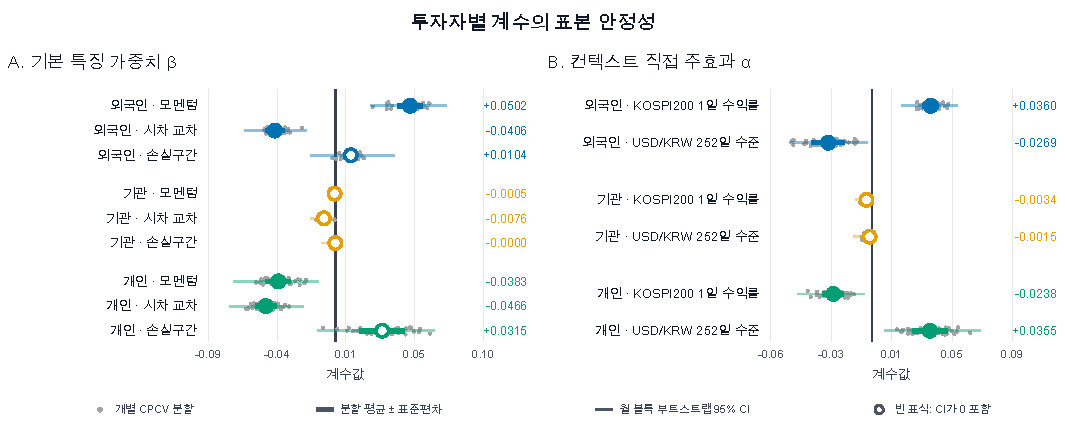
\includegraphics[width=\textwidth]{figures/fig4p_forest_no_v5.pdf}
  \caption{복원된 계수의 표본 안정성. 회색 점은 45개 CPCV 분할, 굵은 선은 분할 간
  표준편차, 가는 선은 달력월 블록 부트스트랩 95\% 신뢰구간이다. 속이 빈 표식은
  신뢰구간이 0을 포함하는 항이며, 오른쪽 값은 분할 평균계수다.}
  \Description{두 패널의 forest plot. 왼쪽은 세 유형의 모멘텀, 시차 교차수급,
  손실구간 계수를, 오른쪽은 KOSPI 200과 환율 직접효과를 보인다. 외국인과 개인의
  계수는 반대 부호이고 대부분의 기관 계수는 0에 가깝다.}
  \label{fig:forest}
\end{figure*}

\begin{table}[t]
  \caption{CPCV 표본외 성능(45개 분할의 평균 $\pm$ 표준편차). 지표는 예측 연관을
  요약하며, 거래가치나 다른 예측모형에 대한 우위를 입증하지 않는다.}
  \label{tab:performance}
  \small
  \centering
  \begin{tabular}{@{}lccc@{}}
    \toprule
    지표 & 외국인 & 기관 & 개인 \\
    \midrule
    방향 정확도 & $0.636\pm0.040$ & $0.536\pm0.035$ & $0.602\pm0.044$ \\
    상관계수      & $0.279\pm0.106$ & $0.060\pm0.062$ & $0.239\pm0.116$ \\
    MAE           & $0.195$ & $0.095$ & $0.266$ \\
    표본외 $R^2$  & $0.105$ & $0.002$ & $0.102$ \\
    \bottomrule
  \end{tabular}
\end{table}

\begin{figure*}[t]
  \centering
  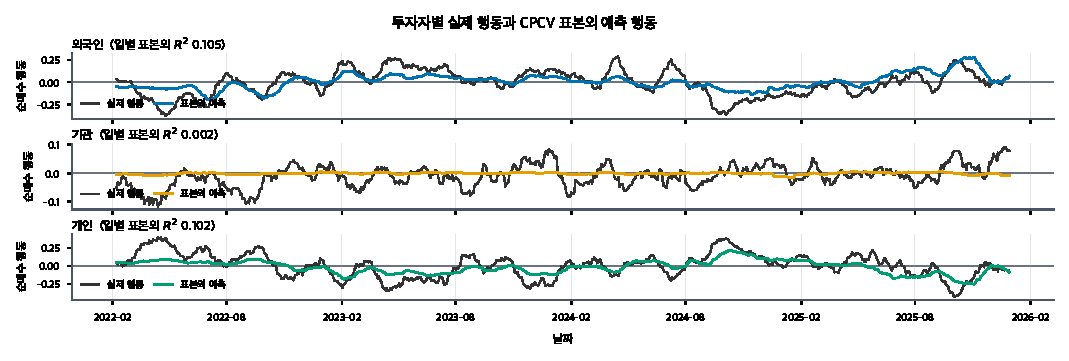
\includegraphics[width=\textwidth]{figures/fig4p_prediction.pdf}
  \caption{투자자 유형별 실제 행동과 CPCV 표본외 예측. 날짜별로 이용 가능한 9개 CPCV
  시험예측을 먼저 평균한 뒤 실제값과 예측값 모두에 20거래일 이동평균을 적용했다.
  패널의 표본외 $R^2$는 평활 전 일별 예측의 45개 분할 평균이며
  표~\ref{tab:performance}와 같다.}
  \Description{외국인, 기관, 개인의 순매수 행동과 표본외 예측을 겹친 세 시계열 패널.
  외국인과 개인 예측은 넓은 수급 국면을 따라가지만 기관 예측은 0 부근에서 평탄하다.}
  \label{fig:prediction}
\end{figure*}

결과는 안정적인 외국인--개인 대비와 낮은 기관 예측력을 보인다. 표~\ref{tab:performance}의
분할 간 산포 때문에 단일 분할로 결론내릴 수 없다. 외국인과 개인 예측은 넓은 수급
국면을 따라가지만 기관 예측은 0 부근에 머문다(그림~\ref{fig:prediction}).
그림~\ref{fig:forest}는 이에 대응하는 계수 안정성을 보인다.

\textbf{(V1)} 외국인 모멘텀 가중치는 $+0.0502$로 45개 분할 모두에서 양수이고, 개인
가중치는 $-0.0383$으로 모든 분할에서 음수다. 시차 교차수급 계수는 세 유형의 모든
분할에서 음수다. 개인 손실구간 계수는 97.8\%의 분할에서 양수다. 기관의 경우 Lasso가
모멘텀과 손실구간 계수를 45개 분할 중 각각 36개와 44개에서 정확히 0으로 만든다.

\textbf{(V2)} 부트스트랩 구간이 0을 제외하는 계수는 여덟 개다. 외국인과 개인 각각의
모멘텀, 시차 교차수급, 두 컨텍스트 직접효과가 이에 해당한다. 개인 손실구간 구간은
$-0.0122$에서 $+0.0665$이고, 모든 기관 구간은 0을 포함한다. 개인 손실구간 계수는
45개 CPCV 분할에서 부호가 완전히 일관되지만 달력월 재표집의 5.5\%에서는 부호가
바뀐다. 따라서 관측을 공유하는 CPCV의 부호 일관성만으로는 불확실성을 과소평가한다.

\textbf{(V3)} 확장형 워크포워드 성능은 창별로 크게 변한다. 외국인 방향 정확도는
$0.610\pm0.116$, 상관은 $0.131\pm0.162$로 CPCV 상관의 절반보다 작다. 이를 시간적
일반화의 한계로 보고한다. 계수 경로는 더 안정적이다. 외국인 모멘텀은 10개 창 모두
양수이고 개인 모멘텀은 모두 음수이며 두 경로는 교차하지 않는다. 두 컨텍스트
직접효과에서도 같은 대비가 나타나고 기관 경로는 0 부근에 머문다.

\textbf{(V4)} 외국인과 개인 계수는 $L_1$, $L_2$, 무벌점 추정에서 소수 넷째 자리까지
일치한다. 기관 계수는 벌점에 더 민감하며, 예를 들어 시차 교차수급은 $-0.0076$에서
$-0.0124$로 변한다.

\textbf{강건성.} 망각계수 0.95, 0.98, 0.99와 모멘텀 기간 10, 20, 60의 9개 조합에서
외국인과 개인 모멘텀 계수는 각각 100\% 양수와
음수다. 개인 손실구간 계수는 적어도 91\%에서 양수다. 모든 유형에 공통 $\lambda$를
적용해도 이러한 부호 판정은 유지된다.

% =====================================================================
\FloatBarrier
\subsection{해석}
\label{sec:interpretation}

\begin{itemize}
\item \textbf{외국인은 시장 방향 및 환율 국면과 안정적인 조건부 연관을 보인다.}
모멘텀 가중치 $+0.0502$는 45개 CPCV 분할 모두에서 양수이고 달력월 부트스트랩
구간도 0을 제외한다. 따라서 최근 가격상승과 외국인 순매수의 양의 연관은 분할 및
재표집 방식에 민감하지 않다. KOSPI 200 효과 $+0.0360$과 환율효과 $-0.0269$도 같은
검증을 통과한다. 다른 특징을 통제하면 시장 상승일의 외국인 순매수는 더 크고, 원화가
직전 252일보다 약할 때는 더 작다. 이 부호는 외국인 추세거래 문헌과 일치한다
~\cite{grinblatt2000investment,choe1999foreign}. 분리되지 않은 상대방 수급과 공통
시장충격 때문에 이를 구조적 선호나 반군집행동으로 해석할 수는 없다.

\item \textbf{개인은 반대 방향의 시장 연관과 더 약한 손실구간 신호를 보인다.}
개인의 모멘텀은 $-0.0383$, KOSPI 200 효과는 $-0.0238$, 환율효과는 $+0.0355$로
외국인과
반대 부호다. CPCV, 달력월 재표집, 워크포워드, 벌점 대체에서 이 대비가 유지된다.
따라서 조건부 개인 순매수는 종목 및 시장 상승 후 더 작고 원화약세 국면에서 더 크다.
강한 음의 동일일 수급상관 때문에 이를 구조적인 개인 역추세 선호로 해석할 수 없다.
손실구간 가중치 $+0.0315$는 CPCV 분할의 97.8\%, 강건성 사양의 최소 91\%에서 양수다.
평균단가 대비 손실이 클수록 순매수가 늘거나 매도가 줄어드는 연관은 손실실현 회피 또는
물타기와 부호가 일치한다. 그러나 달력월 구간은 0을 포함하고, 집계 수급으로는 추가
매수와 매도 연기를 구별할 수 없다. 따라서 이를 손실회피의 직접 증거가 아닌 반복
관측되지만 제한적인 신호로 해석한다.

\item \textbf{집계 기관 수급에서는 안정적인 공통 행동가중치가 나타나지 않는다.}
한국의 집계 ``기관'' 범주에서 지정된 특징은 안정적인 공통 거래규칙을 형성하지 않는다.
주요 계수의 불안정성과 표본외 $R^2=0.002$는 서로 다른 기관 반응이 집계 과정에서
상쇄된다는 해석과 일치한다.
\end{itemize}

% =====================================================================
\subsection{한계}
\label{sec:limitations}

\textbf{(1) 해석 범위.} 복원 가중치는 인과효과가 아니라 조건부 연관이다. 모형에는
수익률, 샤프비율, 거래비용이 없으므로 표~\ref{tab:performance}은 거래규칙이나 수급
예측의 우위를 입증하지 않는다. 같은 날 수급의 회계적 상쇄와 공통 시장충격을 별도로
식별하지 않으므로, 외국인과 개인의 반대 계수 및 음의 시차 교차수급 계수를 독립적
선호로 해석할 수 없다.

\textbf{(2) 처분효과 대용치.} 개인 손실구간 계수는 달력월 블록 부트스트랩을 통과하지
못한다. 또한 평균단가는 계좌별 실현손익이 아니라 집계 거래로 만든 근사치다. 부호는
처분효과와 일치하지만 직접 검정은 아니다.

\textbf{(3) 일반화 가능성.} 단일 종목은 종목 간 이질성을 통제하지만 다른 종목이나
시장에서는 아직 검증되지 않았다.

% =====================================================================
\section{결론}
\label{sec:conclusion}

본 연구는 공통 특징과 모형을 투자자 유형별로 대칭 추정하고 네 가지 안정성 검증을
결합하여, 집계 수급에서 반복되는 조건부 행동계수를 구분했다. 외국인과 개인의
모멘텀ㆍ시장ㆍ환율 계수는 반대 방향이며 표본 구성이 바뀌어도 안정적이었다. 개인
손실구간은 손실실현 회피와 부호가 일치하는 제한적 신호를 유지했지만, 집계 기관
수급에서는 안정적인 공통 행동규칙이 나타나지 않았다. 다만 이 결과는 구조적 선호가
아니라 단일 종목의 조건부 연관이며, 독립적 선호ㆍ상대방 흡수ㆍ공통충격을 분해하지
못한다.

향후에는 외국인 지분율과 유동성이 다른 종목에 같은 추정량과 V1--V4를 적용하여
횡단면 일반화를 검증할 수 있다. 또한 동시 수급의 회계적 상쇄와 각 유형의 직접 반응을
구분할 수 있는 자료와 식별설계가 필요하다. 마지막으로 KRX의 세분 투자자 범주에 대칭
추정을 적용하면 집계가 기관 계수의 불안정성을 만든다는 가설을 직접 검정할 수 있다.


\bibliographystyle{ACM-Reference-Format}
\bibliography{paper-ko,paper-refs-additional}

\end{document}
